% Chapter 11 -- Verilog I: describing hardware
\chapter{Verilog I: describing hardware}\label{ch:verilog1}

Chapters 8--10 used Verilog where it was needed; this chapter teaches it
as a language. The single idea underneath everything: \emph{Verilog
describes hardware, it does not give orders}. Once that lands, the
syntax is small --- two kinds of signals, two recipes for
\texttt{always}, one rule about \texttt{=} versus \texttt{<=}, and a
testbench that is itself just a module. After this chapter you can write
a legal module three different ways, spot the two classic wrong ways,
run it under Icarus Verilog, and read the waveform it produces.

% from-zero:begin
\begin{rulebox}[Before you start]
Chapters~8--10. \emph{Recap:} Verilog describes hardware that exists all at once, not instructions that run in order. If you know a programming language, forget the habit of reading top to bottom.
\end{rulebox}
\begin{wins}[After this chapter you can]
\begin{itemize}
\item describe a combinational and a sequential block in Verilog;
\item explain blocking versus non-blocking assignment and use each correctly;
\item write a testbench and read the waveform in GTKWave;
\item avoid the classic synthesis mistakes.
\end{itemize}
\end{wins}
\begin{principle}[How to think about this]
Hardware description is a different way of thinking from programming: everything you write exists at once and works in parallel. Ask of every line, ``what wires and gates is this?'' not ``what runs next?'' A testbench is your lab bench, so write it before you trust the design.
\end{principle}
% from-zero:end

\section{HDL is not a program}\label{sec:hdlmind}

\index{hardware description language}\index{HDL|see{hardware description
language}} A \emph{hardware description language}\index{Verilog} (HDL)
writes down a circuit. When you write \texttt{assign y = a \& b;} you
are not instructing a machine to AND anything --- you are asserting
that an AND gate exists between \texttt{a}, \texttt{b} and \texttt{y},
now and forever. Statements run whenever their inputs change, all of
them, all the time. There is no ``next line'' because there are no
lines: there is silicon-shaped text.

The reset that makes Verilog readable: \emph{before writing any code,
draw the circuit}. If you cannot point at a gate, a mux or a flip-flop
for a line of code, the line is probably describing software.

\begin{principle}[Code is a schematic written sideways]
Every synthesizable line should map to a part you could sketch:
an \texttt{assign} is wires and gates, a clocked \texttt{always} is
flip-flops, an \texttt{if} inside \texttt{@(*)} is a mux. When a line
has no picture, delete the line, not the picture.
\end{principle}

\section{Modules, ports, wires and regs}\label{sec:ports}

A \emph{module}\index{module (Verilog)} is the unit of hardware: a box
with named connections. \emph{Ports}\index{port (Verilog)} are the box's
boundary wires --- \texttt{input}, \texttt{output}, rarely
\texttt{inout}. Inside, two kinds of signal matter:

\begin{description}
\item[\texttt{wire}] a connection. Driven by \texttt{assign} or by a
port; holds nothing itself. The default: any name you use but never
declare is an implicit wire (declare anyway --- implicit wires hide
typos).
\item[\texttt{reg}] assigned inside an \texttt{always} block. The name
is a lie the language kept: a \texttt{reg} does \emph{not} imply a
register. In a combinational \texttt{@(*)} block it is still just
gates; only an edge-triggered block makes it a real flip-flop.
\end{description}

\begin{figure}[htbp]
\centering
% fig_wires.tex -- wire vs reg, and module hierarchy
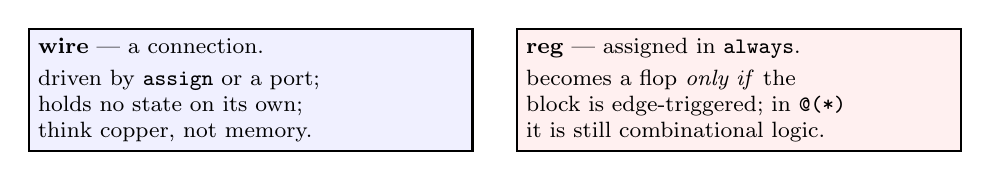
\begin{tikzpicture}[font=\footnotesize]
  \node[draw, thick, fill=blue!6, text width=5.4cm, align=left] at (0,0)
    {\textbf{wire} --- a connection.\\[2pt]
     driven by \texttt{assign} or a port;\\
     holds no state on its own;\\
     think copper, not memory.};
  \node[draw, thick, fill=red!6, text width=5.4cm, align=left] at (6.2,0)
    {\textbf{reg} --- assigned in \texttt{always}.\\[2pt]
     becomes a flop \emph{only if} the\\
     block is edge-triggered; in \texttt{@(*)}\\
     it is still combinational logic.};
\end{tikzpicture}

\caption{Wire vs reg at a glance. Notice the trap in the right card:
\texttt{reg} is a typing rule, not a memory claim --- the block's
sensitivity list decides what silicon you get. Regenerate:
\ttfamily figures/ch11/fig\_wires.tex.}
\label{fig:wires}
\end{figure}

\begin{figure}[htbp]
\centering
% fig_module.tex -- a module as a box of ports
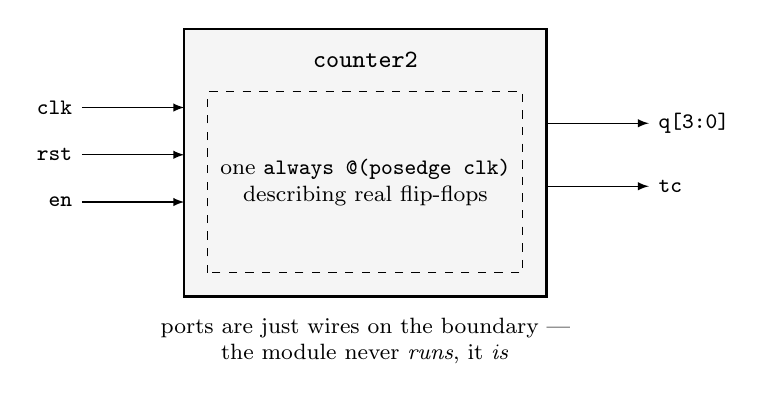
\begin{tikzpicture}[font=\small, >=latex]
  \draw[thick, fill=gray!8] (0,0) rectangle (4.6,3.4);
  \node at (2.3,3.0) {\ttfamily counter2};
  \draw[thin, dashed] (0.3,0.3) rectangle (4.3,2.6);
  \node[align=center, font=\footnotesize] at (2.3,1.45)
    {one \texttt{always @(posedge clk)}\\ describing real flip-flops};
  % input ports
  \foreach \y/\n in {2.4/clk, 1.8/rst, 1.2/en}{
    \draw[->] (-1.3,\y) -- (0,\y);
    \node[left, font=\ttfamily\footnotesize] at (-1.3,\y) {\n}; }
  % output ports
  \foreach \y/\n in {2.2/q[3:0], 1.4/tc}{
    \draw[->] (4.6,\y) -- (5.9,\y);
    \node[right, font=\ttfamily\footnotesize] at (5.9,\y) {\n}; }
  \node[align=center, font=\footnotesize, anchor=north] at (2.3,-0.15)
    {ports are just wires on the boundary ---\\ the module never \emph{runs}, it \emph{is}};
\end{tikzpicture}

\caption{Our counter as a box of ports. Notice that the port list is the
whole contract --- everything inside the dashed boundary is private
machinery. Regenerate: \ttfamily figures/ch11/fig\_module.tex.}
\label{fig:module11}
\end{figure}

\section{\texttt{assign}: combinational logic, permanently}
\label{sec:assign}

\texttt{assign y = expr;} is a permanent connection\index{assign
(Verilog)}: whenever \texttt{expr}'s inputs move, \texttt{y} follows,
in zero simulated time. It is the right home for single expressions
--- muxes as ternaries, logic as boolean expressions, buses split and
joined with \texttt{\{\}} concatenation and \texttt{[hi:lo]} slicing.

\section{The two \texttt{always} recipes}\label{sec:always}

The \texttt{always}\index{always block (Verilog)} block runs procedural
code when its sensitivity list fires. Two recipes cover nearly all
legal hardware:

\begin{figure}[htbp]
\centering
% fig_always.tex -- the two always-block recipes side by side
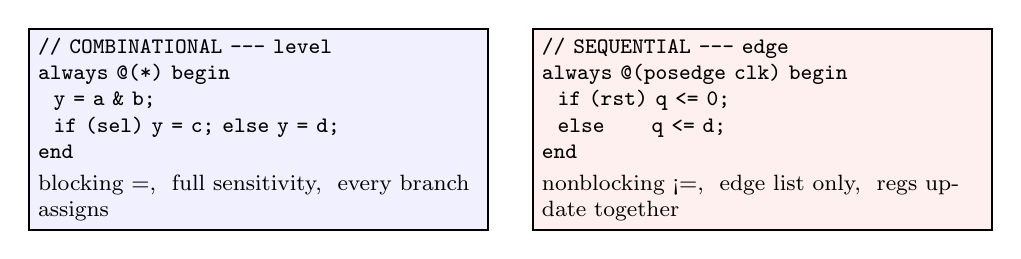
\begin{tikzpicture}[font=\small]
  \node[draw, thick, fill=blue!6, text width=5.6cm, align=left,
        font=\ttfamily\footnotesize, anchor=north west] at (0,0)
    {// COMBINATIONAL --- level\\
     always @(*) begin\\
     \ \ y = a \& b;\\
     \ \ if (sel) y = c; else y = d;\\
     end\\[2pt]
     \textrm{\footnotesize blocking =,\ \ full sensitivity,\ \ every branch assigns}};
  \node[draw, thick, fill=red!6, text width=5.6cm, align=left,
        font=\ttfamily\footnotesize, anchor=north west] at (6.4,0)
    {// SEQUENTIAL --- edge\\
     always @(posedge clk) begin\\
     \ \ if (rst) q <= 0;\\
     \ \ else\ \ \ \ \ \ q <= d;\\
     end\\[2pt]
     \textrm{\footnotesize nonblocking <=,\ \ edge list only,\ \ regs update together}};
\end{tikzpicture}

\caption{The two recipes. Notice the three differences that matter:
the sensitivity list (everything vs.\ one edge), the assignment
(= vs.\ <=), and the duty (assign on every branch vs.\ registers that
keep their value). Regenerate: \ttfamily figures/ch11/fig\_always.tex.}
\label{fig:always}
\end{figure}

\textbf{Combinational} --- \texttt{always @(*)}: full sensitivity,
blocking \texttt{=}, and \emph{every path must assign every variable}.
Miss a branch and the simulator keeps the old value --- you have
described a latch (the wrong-way demo shows it caught red-handed).

\textbf{Sequential} --- \texttt{always @(posedge clk)}: edge
sensitivity only, non-blocking \texttt{<=}, registers keep their value
when unassigned. This is the flip-flop recipe; ch10 built its machines
on it.

\begin{exercise}[easy]
Which recipe is \texttt{always @(a or b) y = a \& b;} and what is wrong
with it?
\end{exercise}

\section{Blocking \texttt{=} vs non-blocking \texttt{<=}}\label{sec:nb}

\index{blocking assignment}\index{non-blocking assignment} One rule to
memorise, then the why.

\begin{rulebox}[The one rule]
Inside \texttt{always @(posedge clk)} use only \texttt{<=}.
Inside \texttt{always @(*)} use only \texttt{=}.
Testbenches may use \texttt{=} anywhere (they are software, on purpose).
\end{rulebox}

The why: \texttt{=} executes in order, immediately; \texttt{<=} queues
the update for the end of the timestep, so every \texttt{<=} sees the
\emph{old} values. That simultaneity is exactly what real flip-flops do
--- at the edge, every D input is sampled at once. Write the pipeline
with \texttt{=} and the second flop sees the \emph{new} value of the
first: two flops collapse into one.

\begin{figure}[htbp]
\centering
% fig_blocking.tex -- blocking vs nonblocking timing cartoon
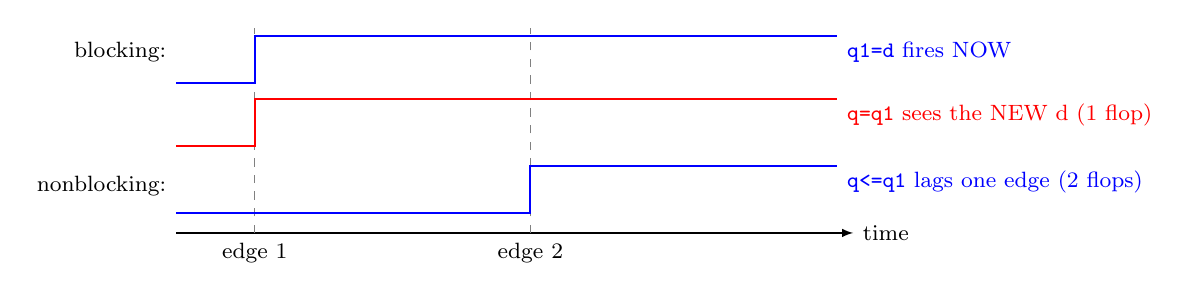
\begin{tikzpicture}[font=\footnotesize, >=latex]
  \draw[->] (0,0) -- (8.6,0) node[right]{time};
  \foreach \x/\l in {1/edge 1, 4.5/edge 2}{
    \draw[dashed, gray] (\x,0) -- (\x,2.6); \node[below] at (\x,0) {\l}; }
  % blocking lane
  \node[left] at (0,2.3) {blocking:};
  \draw[thick, blue] (0,1.9) -- (1,1.9) -- (1,2.5) -- (8.4,2.5);
  \node[right, blue] at (8.4,2.3) {\texttt{q1=d} fires NOW};
  \draw[thick, red] (0,1.1) -- (1,1.1) -- (1,1.7) -- (8.4,1.7);
  \node[right, red] at (8.4,1.5) {\texttt{q=q1} sees the NEW d (1 flop)};
  % nonblocking lane
  \node[left] at (0,0.6) {nonblocking:};
  \draw[thick, blue] (0,0.25) -- (4.5,0.25) -- (4.5,0.85) -- (8.4,0.85);
  \node[right, blue] at (8.4,0.65) {\texttt{q<=q1} lags one edge (2 flops)};
\end{tikzpicture}

\caption{Blocking vs non-blocking on a two-flop pipeline. Notice the
blocking \texttt{q=q1} sees the new \texttt{d} in the same edge ---
the delay element vanished. Regenerate:
\ttfamily figures/ch11/fig\_blocking.tex.}
\label{fig:blocking}
\end{figure}

\section{Parameters and a generate peek}\label{sec:params}

\texttt{parameter}\index{parameter (Verilog)} makes a module
re-usable: width, encodings, divisors. \texttt{generate} loops stamp
out repeated hardware (Chapter 13 uses it to tile a datapath). Both are
elaboration-time --- the parameters are fixed before the circuit
exists, not at run time.

\section{The testbench is a module too}\label{sec:tb}

\index{testbench} A testbench is Verilog used as software on purpose:
it instantiates the \emph{design under test}\index{design under
test|see{DUT}} (DUT), drives \texttt{reg} stimulus, listens on wires,
prints, and calls \texttt{\$finish}. It never synthesizes --- which
frees it to do things hardware can't: \texttt{\$monitor},
\texttt{\$display}, \texttt{\$dumpvars}, file I/O, and \texttt{task}s
like the self-check below.

\section{Icarus + GTKWave: the loop}\label{sec:icarus}

\index{Icarus Verilog} The loop is three commands: \texttt{iverilog}
compiles to a sim model, \texttt{vvp} runs it, \texttt{\$dumpvars}
records a VCD the wave viewer reads. On this book's box, Icarus is
version 13.0 (stable) --- one version note that bites: declare wires
before use, and keep functions out of \texttt{\$monitor} (a
\texttt{\$display} inside a clocked block does the job).

\begin{figure}[htbp]
\centering
% fig_flow.tex -- the sim -> wave pipeline
\begin{tikzpicture}[font=\footnotesize, >=latex]
  \node[draw, thick, fill=blue!6] (src) at (0,0) {\texttt{mux4.v + mux4\_tb.v}};
  \node[draw, thick, fill=blue!6] (ivl) at (2.9,0) {\texttt{iverilog -o sim}};
  \node[draw, thick, fill=blue!6] (vvp) at (5.6,0) {\texttt{vvp sim}};
  \node[draw, thick, fill=amber!15] (vcd) at (8.4,0) {\texttt{.vcd} + trace};
  \node[draw, thick, fill=good!15] (wave) at (11.2,0) {wave / grep};
  \draw[->] (src) -- (ivl); \draw[->] (ivl) -- (vvp);
  \draw[->] (vvp) -- (vcd); \draw[->] (vcd) -- (wave);
  \node[align=center] at (2.9,-0.9) {compiler: syntax,\\ builds the model};
  \node[align=center] at (8.4,-0.9) {runtime executes\\ \texttt{always/assign} events};
\end{tikzpicture}

\caption{The edit $\to$ compile $\to$ run $\to$ wave pipeline. Notice
where errors can live: \texttt{iverilog} catches syntax, \texttt{vvp}
exposes behavior --- a compiled design can still be wrong.
Regenerate: \ttfamily figures/ch11/fig\_flow.tex.}
\label{fig:flow11}
\end{figure}

\begin{lstlisting}[caption={\ttfamily code/ch11\_Makefile --- the sim
targets used throughout this book.},label={lst:mk}]
SIM = iverilog
all: mux counter traffic
mux:     ; iverilog -o /tmp/mux4_sim ch11_mux4.v ch11_mux4_tb.v  && vvp /tmp/mux4_sim
counter: ; iverilog -o /tmp/cnt2_sim ch11_counter2.v ch11_counter2_tb.v && vvp /tmp/cnt2_sim
wave:    ; iverilog -o /tmp/tr2_sim  ch11_traffic2.v ch11_traffic2_tb.v && vvp /tmp/tr2_sim
traffic: wave
\end{lstlisting}

\section{Reading a waveform}\label{sec:wave}

A waveform pane shows each signal's value versus time. Buses render as
hex bands; single bits as high/low lines; \texttt{x} (unknown) and
\texttt{z} (unconnected) get their own colors --- the first thing to
scan for, because an \texttt{x} early is a missing reset or an
undriven input. We don't ship GTKWave screenshots: Figure~\ref{fig:wave}
is drawn from the VCD the testbench actually produced.

\section{Worked example 1: one mux, four legal ways and two wrong}
\label{sec:we-mux4}

\textbf{Strategy.} The 2:1 mux is the smallest complete module. Write it
with \texttt{assign} (ternary), \texttt{assign} (gates),
\texttt{always} (\texttt{if}), \texttt{always} (\texttt{case}) --- then
commit the two classic sins and let the sim expose them.

\textbf{Solution.}
\begin{lstlisting}[caption={\ttfamily code/ch11\_mux4.v --- four legal
muxes plus the two wrong ones (abridged).},label={lst:mux4}]
module mux_if(sel, a, b, y);
  input sel, a, b; output reg y;
  always @(*)                    // way 3: procedural if
    if (sel) y = b; else y = a;
endmodule
module mux_latch(sel, a, b, y);  // WRONG: no else -> inferred latch
  input sel, a, b; output reg y;
  always @(*)
    if (sel == 1'b0) y = a;
endmodule
module mux_stale(sel, a, b, y);  // WRONG: sel missing from sensitivity
  input sel, a, b; output reg y;
  always @(a or b)
    y = sel ? b : a;
endmodule
\end{lstlisting}

\begin{lstlisting}[caption={Real run of \ttfamily ch11\_mux4\_tb.v.
Notice t=10: the legal muxes go to \texttt{b=1}, the latch and the
stale copy stay at 0 --- the two bugs caught in one row each.},
abovecaptionskip=0pt]
t= 0 sel=0 a=0 b=1 | y1..4=0000 latch=0 stale=0
t=10 sel=1 a=0 b=1 | y1..4=1111 latch=0 stale=0
t=20 sel=1 a=1 b=0 | y1..4=0000 latch=0 stale=0
t=30 sel=0 a=1 b=0 | y1..4=1111 latch=1 stale=0
\end{lstlisting}

At t=10 the latch holds its old value instead of following
\texttt{sel}; at t=30 the stale mux missed the \texttt{sel} edge
entirely. Both are ``legal Verilog'' --- the language can't refuse them
because they describe real (unwanted) hardware.

\section{Worked example 2: a counter with a self-checking testbench}
\label{sec:we-counter2}

\textbf{Strategy.} A tb that only prints waveforms makes you the check
--- slow and error-prone. Write the check \emph{into} the tb: a
\texttt{task} comparing reality to expectation, errors counted, a final
PASS/FAIL verdict.

\textbf{Solution.}
\begin{lstlisting}[caption={\ttfamily code/ch11\_counter2\_tb.v ---
the check task and the three assertions.},label={lst:tb2}]
task check(input [3:0] want, input [8*24-1:0] what);
  if (q !== want) begin
    errors = errors + 1;
    $display("FAIL t=%0d %0s: q=%0d expected %0d", $time, what, q, want);
  end
endtask
initial begin
  #12 rst=0; en=1;
  repeat (4) @(posedge clk); #1 check(4, "counted to 4");
  en=0; @(posedge clk); #1 check(4, "hold when en=0");
  rst=1; @(posedge clk); #1 check(0, "rst clears");
  if (errors == 0) $display("PASS: all %0d checks", 3);
  else $display("FAIL: %0d errors", errors);
  $finish;
end
\end{lstlisting}

\begin{lstlisting}[caption={Real output --- and proof the checker
bites: the second run compiles the same tb with \texttt{-DSABOTAGE},
planting one wrong expectation on purpose.},abovecaptionskip=0pt]
PASS: all 3 checks
\end{lstlisting}
\begin{lstlisting}[caption={The sabotaged run --- \texttt{FAIL} lines
name the check, the value, and the expectation.},abovecaptionskip=0pt]
FAIL t=56 planted bad check: q=4 expected 9
FAIL: 1 errors
\end{lstlisting}

The \texttt{\#1} after each edge matters: it waits one timestep so the
non-blocking updates settle before \texttt{check} reads \texttt{q} ---
sample at the same instant and you read the old register value.

\section{Worked example 3: the traffic FSM, re-coded in this chapter's
style}\label{sec:we-traffic2}

\textbf{Strategy.} Take ch10's traffic machine and rewrite it with
\texttt{parameter} encodings and named wires, dump a real VCD, then
read the waveform one transition at a time.

\textbf{Solution.}
\begin{lstlisting}[caption={\ttfamily code/ch11\_traffic2.v ---
parameters carry the encodings; the three blocks stay separate.},
label={lst:tr2}]
parameter RED=2'b00, YEL=2'b01, GRN=2'b10;
parameter NSG=0, NSY=1, EWG=2, EWY=3;
reg [1:0] st, nx;
always @(*) case (st)                 // next-state logic
  NSG: nx = NSY;  NSY: nx = EWG;
  EWG: nx = EWY;  default: nx = NSG;
endcase
always @(posedge clk)                 // state register
  if (rst) st <= NSG; else st <= nx;
always @(*) case (st)                 // output logic (Moore)
  NSG: begin ns=GRN; ew=RED; end
  // ... same shape for NSY, EWG, EWY
endcase
\end{lstlisting}

\begin{lstlisting}[caption={The real trace. Read it like the waveform:
each \texttt{st} edge also updates \texttt{nx} combinationally, so the
``next'' column always shows where the machine will land.},
abovecaptionskip=0pt]
t= 5 rst=1 | st=0 nx=1 | ns=10 ew=00
t=15 rst=0 | st=1 nx=2 | ns=01 ew=00
t=25 rst=0 | st=2 nx=3 | ns=00 ew=10
t=35 rst=0 | st=3 nx=0 | ns=00 ew=01
t=45 rst=0 | st=0 nx=1 | ns=10 ew=00
\end{lstlisting}

\begin{figure}[htbp]
\centering
% fig_wave.tex -- waveform pane from the real VCD rows (like GTKWave)
\begin{tikzpicture}[font=\footnotesize]
\begin{axis}[width=12.4cm, height=6.4cm, xlabel={time (ns)},
  xmin=0, xmax=66, ymin=-0.3, ymax=4.9,
  ytick={0.4,1.4,2.4,3.4,4.4},
  yticklabels={ew,ns,st,nx,rst},
  y tick label style={font=\ttfamily\footnotesize},
  x tick label style={font=\footnotesize}, grid=both, grid style={gray!20}]
\addplot[const plot, very thick, accent] table[x=t, y expr=0.4+\thisrow{ew}*0.22] {figures/ch11/ch11_traffic.dat};
\addplot[const plot, very thick, good] table[x=t, y expr=1.4+\thisrow{ns}*0.22] {figures/ch11/ch11_traffic.dat};
\addplot[const plot, very thick, blue] table[x=t, y expr=2.4+\thisrow{st}*0.22] {figures/ch11/ch11_traffic.dat};
\addplot[const plot, very thick, slate] table[x=t, y expr=3.4+\thisrow{nx}*0.22] {figures/ch11/ch11_traffic.dat};
\addplot[const plot, very thick, red] table[x=t, y expr=4.4+\thisrow{rst}*0.66] {figures/ch11/ch11_traffic.dat};
\draw[dashed, slate] (axis cs:15,-0.2) -- (axis cs:15,4.9);
\node[anchor=west, font=\footnotesize, align=left] at (axis cs:16,4.2)
  {rst releases; st walks\\ 1→2→3→0, nx one ahead};
\end{axis}
\end{tikzpicture}

\caption{The same run as a waveform pane (drawn from the VCD rows).
Notice \texttt{nx} always sits one state ahead of \texttt{st} --- the
register/combinational split made visible. Regenerate:
\ttfamily figures/ch11/fig\_wave.tex\ + code/ch11\_traffic2.vcd.}
\label{fig:wave}
\end{figure}

Line by line: t=5 the first edge loads \texttt{st=NSG}, outputs
\texttt{ns=GRN ew=RED} appear combinationally; t=15 reset releases and
the edge steps \texttt{st} to \texttt{NSY}; every 10\,ns another edge
walks the cycle.

\section{Worked example 4: the pipeline that ate a flop}
\label{sec:we-pipe}

\textbf{Strategy.} Prove the \texttt{=}/\texttt{<=} rule is real
silicon, not style: simulate a two-flop pipeline written both ways and
count effective delay elements.

\textbf{Solution.}
\begin{lstlisting}[caption={Real run of \ttfamily ch11\_pipe\_tb.v.
Notice t=15: \texttt{q\_block} is already 1 while the nonblocking
\texttt{q\_nb} still holds 0 --- blocking leaked \texttt{d} through two
``flops'' in one edge. The nonblocking output arrives at t=25, a full
edge later, as real hardware would.},abovecaptionskip=0pt]
t= 5 clk=1 d=0 | q_nb=x q_block=0
t=15 clk=1 d=1 | q_nb=0 q_block=1
t=25 clk=1 d=1 | q_nb=1 q_block=1
t=45 clk=1 d=0 | q_nb=1 q_block=0
\end{lstlisting}

With \texttt{=}, \texttt{q1=d} completes \emph{before} \texttt{q=q1}
runs, so \texttt{q} receives the brand-new \texttt{d} --- the
simulation shows a one-flop pipeline. Synthesis tools may or may not
reorder this; never rely on it. With \texttt{<=} both assignments read
the old values: two edges, two flops.

\section{Worked example 5: one name, N flip-flops}
\label{sec:we-gen}

\textbf{Strategy.} Show \texttt{parameter} + \texttt{generate} paying
rent: instantiate the same \texttt{regN} at width 4 and width 8, feed
them a shared bus, and watch each keep its own slice.

\textbf{Solution.}
\begin{lstlisting}[caption={\ttfamily code/ch11\_gen.v --- the
generate loop stamps out N posedge always blocks.},label={lst:gen}]
module regN #(parameter N = 4) (clk, d, q);
  input clk; input [N-1:0] d; output reg [N-1:0] q;
  genvar i;
  generate
    for (i = 0; i < N; i = i + 1) begin : ff
      always @(posedge clk) q[i] <= d[i];
    end
  endgenerate
endmodule
\end{lstlisting}

\begin{lstlisting}[caption={Real run --- \texttt{q4} tracks
\texttt{d[3:0]}, \texttt{q8} the full byte, each through its own
generated flops.},abovecaptionskip=0pt]
t=12 d=10110100 | q4=0100 q8=10110100
t=24 d=01101001 | q4=1001 q8=01101001
\end{lstlisting}

The loop body is not a runtime loop --- it is a cookie cutter pressed
$N$ times before simulation even starts.

\section{Summary}

\begin{center}
\begin{tabularx}{\textwidth}{l>{\raggedright\arraybackslash}X}
\toprule
\textbf{Construct} & \textbf{Use it for / the rule to remember}\\
\midrule
\texttt{wire} & connections; driven by \texttt{assign}/ports\\
\texttt{reg} & assigned in \texttt{always}; a flop only on an edge\\
\texttt{assign} & one permanent combinational expression\\
\texttt{always @(*)} & combinational; \texttt{=}; every branch assigns\\
\texttt{always @(posedge clk)} & sequential; \texttt{<=}; regs hold
otherwise\\
\texttt{parameter} & elaboration-time constants (width, encodings)\\
\texttt{generate} & stamps repeated hardware before sim/synth\\
testbench & a module that is software: monitor, check, dump, finish\\
\texttt{x}/\texttt{z} & unknown / undriven --- read them first on any
waveform\\
\bottomrule
\end{tabularx}
\end{center}

\section{Common mistakes}\label{sec:cm11}

\begin{tripwire}[Writing software-style sequential Verilog]
Loops and ``next lines'' belong to programs. If your module has a
\texttt{for} outside \texttt{generate} or an algorithm's worth of
variables, you are writing code for a machine that doesn't exist ---
draw the hardware first.
\end{tripwire}
\begin{tripwire}[\texttt{=} where \texttt{<=} belongs]
Blocking inside a posedge block makes reads see new values ---
pipelines collapse, and synthesis may not save you
(\S\ref{sec:we-pipe} has the proof on tape). The rule takes one line:
edge blocks get \texttt{<=}.
\end{tripwire}
\begin{tripwire}[Describing hardware you cannot draw]
If a line has no corresponding gate or flop in your sketch, it is not
hardware --- it is a wish. The missing \texttt{else} that infers a
latch (\S\ref{sec:we-mux4}) is the canonical example.
\end{tripwire}
\begin{tripwire}[Half a sensitivity list]
\texttt{always @(a or b)} with \texttt{sel} inside the expression
ignores \texttt{sel} edges --- the wrong-way demo caught it holding a
stale output. Use \texttt{@(*)} and let the tool list the signals.
\end{tripwire}
\begin{tripwire}[A testbench that only watches]
A tb without checks makes you the diff. One \texttt{task} and an error
counter turns every run into a verdict
(\S\ref{sec:we-counter2}); \texttt{-DSABOTAGE} proves the checker
bites.
\end{tripwire}

\begin{exercise}[medium]
Predict before running: for \texttt{mux\_stale}, what does \texttt{y}
show if \texttt{sel} toggles twice with \texttt{a}, \texttt{b} fixed?
Sketch the expected line, then check against
\S\ref{sec:we-mux4}'s table.
\end{exercise}

\begin{exercise}[medium]
The \texttt{check} task reads \texttt{q} one \texttt{\#1} after the
edge. What goes wrong if the \texttt{\#1} is removed, and which
assignment rule makes it go wrong?
\end{exercise}

\begin{exercise}[hard]
Write a testbench for ch9's \texttt{adder4}: drive all 256 operand
pairs, compare against \texttt{a+b} computed in the tb, print only the
verdict.
\end{exercise}

\section*{Additional exercises}
\addcontentsline{toc}{section}{Additional exercises}

\begin{exercise}[easy]
Wire or reg? Classify: a port driven by a submodule; a counter's
\texttt{q}; a tb's clock; a mux's select line.
\end{exercise}
\begin{exercise}[easy]
Write the two \texttt{always} recipe headers from memory, then say
which two choices each recipe fixes.
\end{exercise}
\begin{exercise}[easy]
What do \texttt{x} and \texttt{z} mean on a waveform, and which usually
points at a missing reset?
\end{exercise}
\begin{exercise}[easy]
Order the pipeline commands: \texttt{vvp}, \texttt{\$dumpvars},
\texttt{iverilog}, \texttt{\$finish}.
\end{exercise}
\begin{exercise}[medium]
Rewrite \texttt{mux\_case} as a 4:1 mux with \texttt{sel[1:0]}; name
the one change that makes it latch-free.
\end{exercise}
\begin{exercise}[medium]
Fix this testbench: it declares \texttt{wire clk;} and tries
\texttt{always \#5 clk = \textasciitilde clk;}. What does the compiler
say, and what's the minimal change?
\end{exercise}
\begin{exercise}[medium]
Predict the waveform: \texttt{always @(posedge clk) begin q <= d;
q2 <= q; end} --- sketch \texttt{d}, \texttt{q}, \texttt{q2} for four
edges, then verify in sim.
\end{exercise}
\begin{exercise}[medium]
The sabotage run used \texttt{-DSABOTAGE}. Write the tb line that would
count checks automatically (so \texttt{PASS: all 3} needs no hardcoded
3).
\end{exercise}
\begin{exercise}[medium]
A teammate's \texttt{@(*)} block assigns \texttt{y} only when
\texttt{en} is 1. Two sentences: what hardware appears, and how do you
confirm it in sim?
\end{exercise}
\begin{exercise}[medium]
Give the \texttt{parameter} list and instantiation lines to reuse
\texttt{counter2} at width 8 without editing its source.
\end{exercise}
\begin{exercise}[medium]
In \S\ref{sec:we-pipe}'s trace, at which time does \texttt{q\_block}
first diverge from \texttt{q\_nb}, and which assignment order produced
it? Explain both columns.
\end{exercise}
\begin{exercise}[hard]
Extend \texttt{traffic2} with a pedestrian input: \texttt{walk} forces
the next state to \texttt{NSY} regardless. Update all three
\texttt{always} blocks and add a tb check that proves the detour.
\end{exercise}
\begin{exercise}[hard]
Self-checking adder tb (the inline exercise) plus one more idea: seed
the stimulus from \texttt{\$random}, run 1000 pairs, report the verdict.
What did randomness buy you?
\end{exercise}
\begin{exercise}[hard]
Implement \texttt{shiftN \#(parameter N)}: an $N$-stage shift register
written \emph{without} generate (one \texttt{always} block, slicing
allowed) and \emph{with} generate; argue which is clearer.
\end{exercise}
\begin{exercise}[hard]
Draw, then describe: a 2-bit saturating counter (counts up to 3 and
sticks, down to 0 and sticks). Write module + tb, self-checking, in
this chapter's style. HDLBits's language track
(\texttt{hdlbits.01xz.net}) drills exactly these patterns.
\end{exercise}

\section*{Hints and answers}
\addcontentsline{toc}{section}{Hints and answers}
\begin{description}
\item[Recipe (easy, inline)] Combinational shape but a half sensitivity
list --- \texttt{sel} missing means stale output; use \texttt{@(*)}.
\item[Classify (easy)] Submodule-driven port: wire; counter q: reg;
tb clock: reg; select line: wire.
\item[Recipes (easy)] \texttt{always @(*)} fixes \texttt{=} + full
sensitivity + every-branch-assigns; \texttt{@(posedge clk)} fixes
\texttt{<=} + edge list + hold-value.
\item[x/z (easy)] Unknown and undriven; \texttt{x} usually points at
the missing reset.
\item[Pipeline order (easy)] \texttt{iverilog} $\to$ \texttt{vvp}
(with \texttt{\$dumpvars} inside the tb) $\to$ wave; \texttt{\$finish}
ends the run.
\item[4:1 mux (medium)] \texttt{case (sel)} over 4 rows +
\texttt{default} --- completeness kills the latch.
\item[Fix the tb (medium)] \texttt{wire clk} can't take procedural
assigns --- the compiler complains about the \texttt{always} drive;
declare \texttt{reg clk}.
\item[Wave predict (medium)] \texttt{q} follows \texttt{d} one edge
late, \texttt{q2} two edges --- a clean 2-deep shift.
\item[Auto-count (medium)] An \texttt{integer n} incremented in
\texttt{check}; print \texttt{n} in the verdict.
\item[Latch confirm (medium)] An inferred latch; drive \texttt{en} low
after a known value and watch \texttt{y} hold it.
\item[Width-8 reuse (medium)] \texttt{counter2 \#(8) u(...)} --- the
\texttt{\#()} syntax overrides \texttt{W} at instantiation.
\item[Pipe divergence (medium)] t=15: \texttt{q1=d} completed before
\texttt{q=q1}, so the new \texttt{d} leaked through in one edge.
\item[Walk detour (hard)] Next-state: \texttt{walk} overrides to
\texttt{NSY}; a tb check waits one edge and asserts
\texttt{st==NSY}.
\item[Random pairs (hard)] Coverage without a hand-picked list ---
corner cases you didn't think to write.
\item[shiftN (hard)] Slicing version is one line
\texttt{q <= \{q[N-2:0], d\}}; generate is clearer when stages differ.
\item[Saturating counter (hard)] Two extra boundary conditions in the
next-state logic; the tb checks both rails.
\end{description}

\section*{Further reading}
\addcontentsline{toc}{section}{Further reading}

\begin{itemize}
\item \emph{ChipVerify Verilog Tutorial},
\url{www.chipverify.com/verilog/verilog-tutorial} --- the
topic order this chapter follows (modules $\to$ assign $\to$ always
$\to$ tb); reference depth per construct, free. Verified 2026-10-11.
\item S.~Williams, \emph{Icarus Verilog} documentation ---
\url{https://steveicarus.github.io/iverilog/} --- the compiler's own
docs incl.\ the v13 quirks we hit ($\$\,$monitor limits, declaration
rules). Verified 2026-10-11.
\item \emph{HDLBits} --- \url{https://hdlbits.01xz.net} --- the
language track is this chapter as drills: small Verilog problems with
instant feedback; do Circuits/Getting Started next. Verified
2026-10-11.
\item Harris \& Harris, \emph{Digital Design and Computer
Architecture}, 2nd ed., ch.~4 --- the textbook's Verilog chapter,
same ``two recipes'' discipline; companion materials at
\url{https://pages.hmc.edu/harris/ddca/}~\cite{ddca}. Verified
2026-10-11.
\item \emph{fpga4fun.com} --- short real projects once the syntax
settles; their ``how FPGA works'' pages bridge this chapter to the
hardware~\cite{fpga4fun}. Verified 2026-10-11.
\item Nisan \& Schocken, \emph{nand2tetris.org/course}, project 3 ---
write the same registers in a second HDL; the concepts transfer
line-for-line. Verified 2026-10-11.
\end{itemize}

\begin{rulebox}[{Watch instead}]
\begin{enumerate}
\item \emph{Icarus Verilog and GTKWave Tutorial} --- Lady Engineer,
10:59, \url{https://www.youtube.com/watch?v=clLL8smqwL0} --- install
to first waveform; matches \S\ref{sec:icarus}--\S\ref{sec:wave}.
Accessed 2026-10-11.
\item \emph{Get Started With FPGAs and Verilog in 13 Minutes!} ---
13:26, \url{https://www.youtube.com/watch?v=aWm9pJ2KobA} --- Verilog
on the Tang Nano 9K board this book uses; matches
\S\ref{sec:hdlmind}--\S\ref{sec:always}. Accessed 2026-10-11.
\item \emph{Introduction to Verilog HDL using Free Software Icarus,
GTKWave, and VS Code} --- boyfriendnibluefairy, 42:03,
\url{https://www.youtube.com/watch?v=vN1wzM0NO4c} --- the long-form
version covering this whole chapter; watch when you want the lecture.
Accessed 2026-10-11.
\end{enumerate}
\end{rulebox}

\section*{Notes}
\addcontentsline{toc}{section}{Notes}

\chapternotes{%
The topic order follows the ChipVerify Verilog tutorial; style rules
(two \texttt{always} recipes, \texttt{=}/\texttt{<=} split) follow
Harris \& Harris ch.~4~\cite{ddca}; practice sets come from
HDLBits~\cite{hdlbits}; the sim toolchain is Icarus Verilog 13.0. All
outputs are verbatim runs on this box: the mux wrong-way table, the
PASS/FAIL checks, the traffic trace, the pipeline-collapse demo, and
the generate run. The waveform figure is regenerated from the actual
VCD/monitor rows (drawn, not a screenshot).}
